\section{Vorlesung 02.12.2016 (Spezialvorlesung 2?)}

\subsection{Cographen \& Cotrees}
\underline{Phylogenetik}
\begin{itemize}
    \item Erforschung von Abstammung
    \item Rekonstruktion von phylogenetischen Bäumen (\glqq{Stammbäume}\grqq )
    \item Speziesbäume/Genbäume
\end{itemize}    
Ergebnisse:
\begin{itemize}
    \item Genverlust (loss)
    \item Aufspaltung zu einer neuen Spezies (speciation)
    \item Duplikation von Genen (duplication)
    \item horizontaler Gentransfer (HGT)
\end{itemize}
\begin{center}
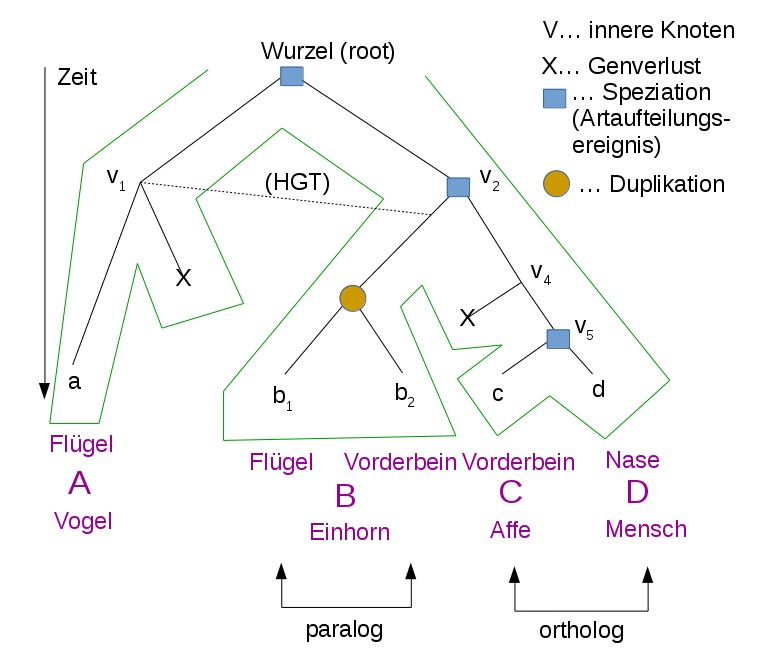
\includegraphics[scale=0.5]{lectures/161202/pix/01.jpg}
\end{center}
\par\medskip
\underline{Def.:} Baum (tree)
\newline
Ein Baum T=(V,E) ist ein zusammenhängender Graph, der keine Kreise enthält (azyklisch).
\par\medskip
\underline{Def.:} Zusammenhang
\newline
Ein Graph G=(V,E) ist zusammenhängend, wenn es zwischen jedem möglichen Paar von Knoten einen Pfad gibt.
\par\medskip
\underline{Theorem:}
\newline
T=$\left(V,E\right)$ ist ein Baum $\Leftrightarrow \exists!$ Pfad zwischen zwei zufällig gewählten Knoten existiert.
($\Leftrightarrow$ … aus dem folgt; $\exists!$ … genau einem)
\par\medskip
\underline{Beweis:}
\newline
$\Rightarrow$ : Da T zusammenhängend ist, gibt es einen Pfad zwischen v, u $\in$ V(T), $\forall$ v, u $\in$ V(T).
Angenommen es gäbe noch einen 2. Pfad, dann gibt es einen Kreis; Widerspruch zur Definition.
\newline
$\Leftarrow$ : Wenn genau ein Pfad existiert, ist T zusammenhängend, Also gibt es auch keine Kreise; T ist ein azyklischer Graph = Baum.
\par\medskip
\underline{Def.:} Distanz
\newline
Die Distanz d(u,v) zwischen zwei Knoten u, v $\in$ V ist gleich der Anzahl der Kanten im kürzesten Pfad zwischen u und v.
\par\medskip
\underline{Def.:} Lowest Common Ancester (lca)
\newline
Seien x,y $\in$ V(T) Blätter im Baum T mit Wurzel r.
Sei $P_x = \{x, x_1 , x_2 , …, r\}$ der Pfad von x nach r und $P_y = \{y, y_1 , y_2 , …, r\}$ der Pfad von y nach r.
Dann $lca (x,y)=min(d(d,v_i), d(y,v_i))$ mit $v_i$ $\in$ ($P_x \cap P_y$)
\newline
$v_i$ … mehrere v's (kann auch r sein)
\newline
r … root (Wurzel)
\begin{itemize}
	\item $P_{{b_2}{r}} = \{b_2, v_3, v_2, r\}$
	\item $P_{dr} = \{d, v_5, v_4, v_2, r\}$
	\item $P_{{b_2}{r}} \cap P_{dr} = \{v_2, r\}$
	\begin{itemize}
		\item $d(b_2, v_2) = 2$
		\item $d(b_2, r) = 3$
	\end{itemize}
\end{itemize}
\underline{Def.:}

\begin{itemize}
	\item Homologie: 2 Gene sind homolog, wenn sie die selben Vorfahren haben
	\item Orthologie: 2 Gene sind ortholog, wenn ihr lca eine Speziation (Artaufteilungsereignis) ist
	\item Paralogie: 2 Gene sind paralog, wenn ihr lca eine Duplikation ist
\end{itemize}
\underline{Def.:} $\Theta$-Relation (Orthologie-Relation)
\newline
Seien x,y $\in$ H, H = Menge von Genen
\newline
(x,y) $\in \Theta \Leftrightarrow$ lca(x,y) ist eine Speziation.
\newline
Diese Relation ist reflexiv (rückbezüglich), symmetrisch, aber \underline{nicht} transitiv (mit sich ziehend).
\newline
Bestimmung von Orthologie:
\begin{itemize}
	\item Sequenzähnlichkeit
	\item Syntenie (\glqq Gemeinsamkeiten in der Reihenfolge von Genen oder Gensegmenten auf verschiedenen chromosomalen Abschnitten. […] ist ein Maß für die genetische Verwandtschaft der beiden Arten.\grqq [Wikipedia])
\end{itemize}
\begin{center}
	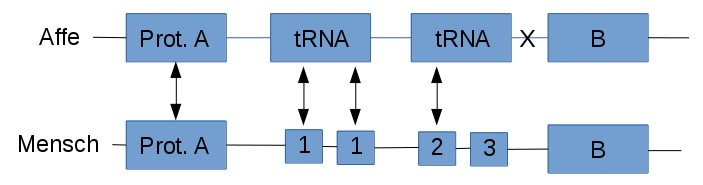
\includegraphics[scale=0.5]{lectures/161202/pix/02.jpg}
\end{center}
z.B. Tool: ProteinOrtho
\par\medskip
\underline{Def.:} $\sim$-Relation (fast-Orthologie)
\newline
(x,y) $\in$ $\sim$, wenn x,y als ortholog eingestuft werden.
\newline
Ziel: Korrigieren $\sim$ sodass wir $\Theta$ erhalten. Dazu stellen wir $\sim$ und $\Theta$ als Graphen dar.
\newline
\begin{tabular}{cccc}
	&$G_{\Theta} = (V_{\Theta} , E_{\Theta})$ & & $G_\sim = (V_\sim, E_\sim)$  \\
	& & $V_\Theta = V_\sim = Gene$ &
\end{tabular}
\newline
\begin{tabular}{cp{1.35cm}c}
	$E_\Theta = \{(x,y) \in {V \choose 2} \mid x \Theta y\}$ & & $E_\sim = \{(x,y) \in {V \choose 2} \mid x \sim y, y \sim x\}$
\end{tabular}
\newline
${V \choose 2}$ … alle möglichen Kombinationen von zwei Knoten
\par\medskip
\underline{Def.:} Komplementgraph (complement)
\newline
Sei G=(V,E) ein Graph. Das Komplement $\overline{G}$ von G ist der Graph $\overline{G} = (V, \overline{E})$ mit $\overline{E} = \{(u,v) \in {V \choose 2} \mid (u,v) \notin E\}$
\begin{center}
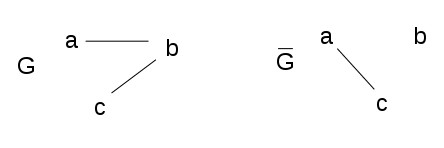
\includegraphics[scale=0.5]{lectures/161202/pix/03.jpg}
\end{center}
\par\medskip
\underline{Def.:} Teilgraph
\newline
Sei G=(V,E) ein Graph und H $\subseteq$ G. H ist Teilgraph von G, wenn V(H) $\subseteq$ V(G), E(H) $\subseteq$ E(G). Ein induzierter Teilgraph ist ein Teilgraph H von G bei dem alle Knoten die in G benachbart sind, auch in H benachbart sein müssen.
\newline
(v,u) $\in$ E(G) $\land$ u,v $\in$ V(H) $\Leftrightarrow$ (v,u) $\in$ E(H)
\newline
$\land$ … Konjunktion
\begin{center}
	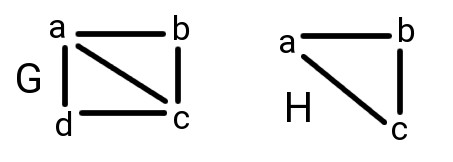
\includegraphics[scale=0.5]{lectures/161202/pix/04.jpg}
\end{center}
\par\medskip
\underline{Def.:} disjunkte Vereinigungen
\newline
Graphen G,H: G+H ist ein Graph mit V(G) $\cup$ V(H) und E(G) $\cup$ E(H).
\begin{center}
	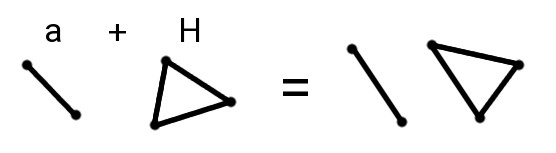
\includegraphics[scale=0.5]{lectures/161202/pix/05.jpg}
\end{center}
\par\medskip
\underline{Def.:} Cograph
\begin{enumerate}
	\item $K_1$ ist ein Cograph 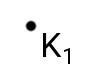
\includegraphics[scale=0.25]{lectures/161202/pix/13.jpg}
	\item G ist ein Cograph $\Leftrightarrow$ $\overline{G}$ ist ein Cograph
	\item G, H sind Cographen $\Leftrightarrow$ G+H ist ein Cograph
\end{enumerate}
Erstellung von Cographen:
\begin{center}
	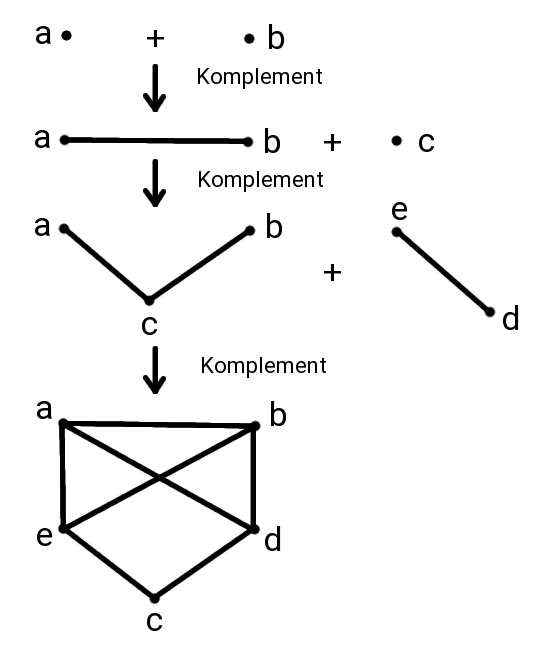
\includegraphics[scale=0.5]{lectures/161202/pix/06.jpg}
\end{center}
Eigenschaften von Cographen:
\newline
Sei G=(V,E) ein Cograph und H $\subseteq$ G,H Cograph
\renewcommand{\labelenumi}{\roman{enumi})}
\begin{enumerate}
	\item G enthält $\underline{keine}$ induzierten $P_4$'s
	\item H ist zusammenhängend $\Leftrightarrow$ $\overline{H}$ ist nicht zusammenhängend
	\item G kann aus einzelnen Knoten ($K_1$) zusammengesetzt werden
\end{enumerate}
\begin{center}
	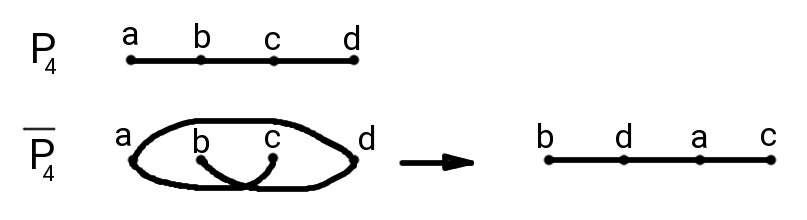
\includegraphics[scale=0.5]{lectures/161202/pix/07.jpg}
\end{center}
$\Rightarrow P_4 = \overline{P_4}$
\newline
Ein Cograph muss jedoch ein $P_4$-freier Graph sein.
\newline
Cograph = $P_4$-free graphs = complement reducible graphs
\par\medskip
Test ob G=(V,E) ein Cograph ist:
\newline
Input: Graph G
\newline
i $\leq$ Cograph (G) \{
\newline
\phantom{}\hspace{1.5cm} if ($\mid V(G)\mid < 4)$ \{return true;\}
\newline
\phantom{}\hspace{1.5cm} c = \{Zusammenhangskomponenten von G\}
\newline
\phantom{}\hspace{1.5cm} if($\mid c \mid $ = 1) \{c'=\{Komponenten von $\overline{G}$\}\}
\newline
\phantom{}\hspace{1.5cm} if ($\mid c'\mid = 1)$ \{return false;\}
\newline
\phantom{}\hspace{1.5cm} else \{
\newline
\phantom{}\hspace{2.5cm} foreach (c $\in$ C)
\newline
\phantom{}\hspace{2.5cm} \{isCograph (c) \}
\newline
\phantom{}\hspace{1.5cm} \}
\newline
\}
\newline
Bei isCograph: je nachdem ob c oder c' rausgekommen ist, muss c oder c' geprüft werden.
\par\medskip
\underline{Theorem:}
\newline
$\sim = \Theta \Leftrightarrow G_\Theta = G_\sim$ und $G_\Theta$ ist ein Cograph
\newline
Damit können wir testen, ob $G_\sim$ ein Orthologiegraph ist.
\newline
Was passiert wenn $\sim \neq \Theta$ bzw. $G_\sim$ kein Graph?
\newline
$\Rightarrow$aktuelle Forschung $\Rightarrow$Es gibt Lösungen $G_\sim$ zu editieren mit optimalen Kriterien, sodass der editierte $G_\sim$ ein Cograph ist. Z.B. ILP (integer linear program), Cograph-editing. Alle Algorithmen, die exakte Möglichkeiten liefern, brauchen sehr lange und sind in der Praxis nicht nutzbar.
\newline
Weitere Literatur: Marc Hellmuth
\par\medskip
\underline{Theorem:}
\newline
Für jeden Cographen gibt es einen eindeutigen Cotree (Cobaum)
\newline
\begin{center}
	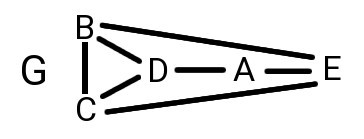
\includegraphics[scale=0.5]{lectures/161202/pix/08.jpg}
\end{center}
\renewcommand{\labelenumi}{\arabic{enumi}.}
\begin{enumerate}
	\item Schritt: Komplement \\
	\begin{center}
		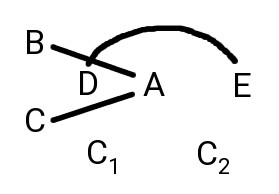
\includegraphics[scale=0.5]{lectures/161202/pix/09.jpg}
	\end{center}
	\item Schritt: umgekehrte disjunkte Vereinigung \\
	\begin{center}
		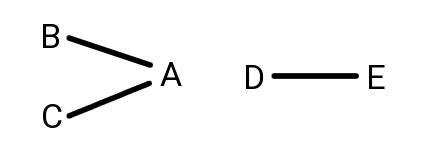
\includegraphics[scale=0.5]{lectures/161202/pix/10.jpg}
		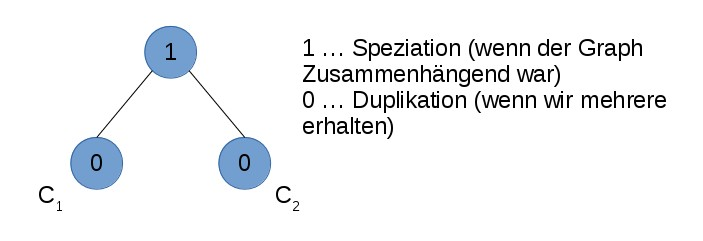
\includegraphics[scale=0.5]{lectures/161202/pix/11.jpg}
	\end{center}
	\item Schritt: Komplement
	\begin{center}
		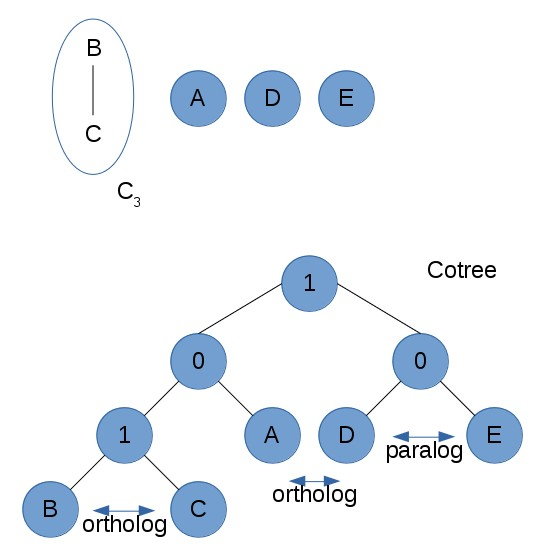
\includegraphics[scale=0.55]{lectures/161202/pix/12.jpg}
	\end{center}
\end{enumerate}